\documentclass[a4paper]{article}
\usepackage{hyperref, hyperlatex, graphicx, color, alltt}
\usepackage{Sweave}
\usepackage[round]{natbib}
\definecolor{Red}{rgb}{0.7,0,0}
\definecolor{Blue}{rgb}{0,0,0.8}
\definecolor{hellgrau}{rgb}{0.55,0.55,0.55}
\newcommand{\pkg}[1]{\texttt{#1}}
\newenvironment{smallexample}{\begin{alltt}\small}{\end{alltt}}

\begin{document}

%\VignetteIndexEntry{Support Vector Machines---the Interface to libsvm in package e1071}
%\VignetteDepends{e1071,rpart,xtable}
%\VignetteKeywords{classification, regression, machine learning, benchmarking, support vector machines}
%\VignettePackage{e1071}


\setkeys{Gin}{width=0.8\textwidth}

\title{Support Vector Machines
  \footnote{A smaller version of this
    article appeared in R-News, Vol.1/3, 9.2001}\\ 
\large The Interface to \texttt{libsvm} in package \pkg{e1071}}
\author{by David Meyer\\
  Technische Universit\"at Wien, Austria\\
\url{David.Meyer@ci.tuwien.ac.at}
}
\maketitle
\sloppy

``Hype or Hallelujah?'' is the provocative title used by
\cite{svm:bennett+campbell:2000} in an overview of Support Vector
Machines (SVM).
SVMs are currently a hot topic in the machine learning community,
creating a similar enthusiasm at the moment as Artificial Neural
Networks used to do before. Far from being a panacea, SVMs yet
represent a powerful technique for
general (nonlinear) classification, regression and outlier detection with an intuitive
model representation.


The package \pkg{e1071} offers an interface to the
award-winning\footnote{The library won the IJCNN 2001 Challenge by solving two of
  three problems: the Generalization Ability Challenge (GAC) and the Text
  Decoding Challenge (TDC). For more information, see: \url{http://www.csie.ntu.edu.tw/~cjlin/papers/ijcnn.ps.gz}.}
C++-implementation by Chih-Chung Chang and Chih-Jen Lin,
\texttt{libsvm} (current version: 2.31), featuring:
\begin{itemize}
\item $C$- and $\nu$-classification
\item one-class-classification (novelty detection)
\item $\epsilon$- and $\nu$-regression
\end{itemize}
and includes:
\begin{itemize}
\item linear, polynomial, radial basis function, and sigmoidal kernels
\item formula interface
\item $k$-fold cross validation
\end{itemize}
For further implementation details on \texttt{libsvm}, see \cite{svm:chang+lin:2001}.

\section*{Basic concept}
SVMs were developed by \cite{svm:cortes+vapnik:1995} for binary
classification. Their approach may be roughly sketched as follows:

\begin{description}
 \item[Class separation:] basically, we are looking for the optimal separating hyperplane
  between the two classes by maximizing the
  \textit{margin} between the classes' closest points (see Figure
  \ref{fig:svm1})---the points lying on the boundaries are called \textit{support vectors}, and
  the middle of the margin is our optimal separating hyperplane;
 \item[Overlapping classes:] data points on the ``wrong'' side
  of the discriminant margin are weighted down to reduce their influence (\textit{``soft margin''});
 \item[Nonlinearity:] when we cannot
  find a \textit{linear} separator, data points are projected into an 
  (usually) higher-dimensional space where the data points effectively
  become linearly separable (this projection is realised via \textit{kernel
    techniques});
 \item[Problem solution:] the whole task can be formulated as a
  quadratic optimization problem which can be solved by known techniques.
\end{description}
\noindent A program able to perform all these tasks is called a \textit{Support
  Vector Machine}.

\begin{figure}[htbp]
  \begin{center}
    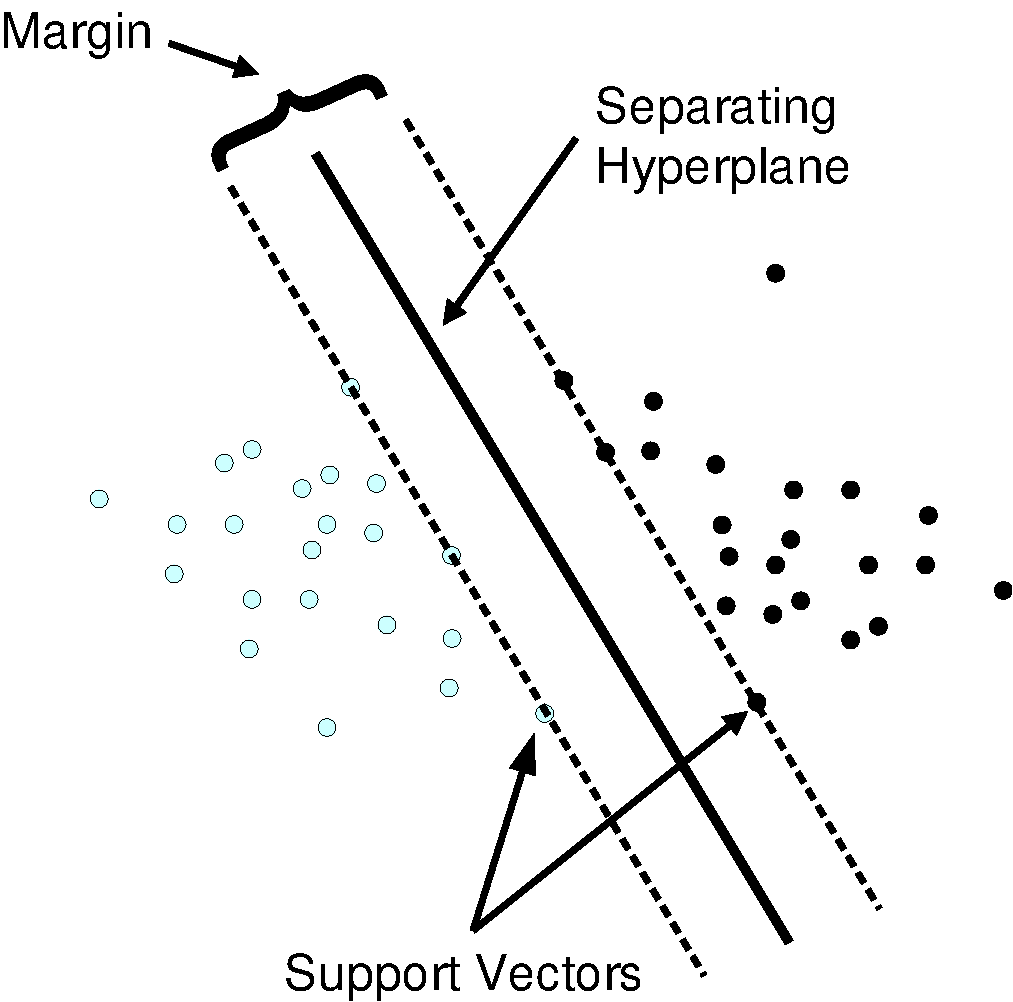
\includegraphics[width=8cm]{svm}
    \caption{Classification (linear separable case)}
    \label{fig:svm1}
  \end{center}
\end{figure}

Several extensions have been developed; the ones currently
included in \texttt{libsvm} are:

\begin{description}
 \item[$\nu$-classification:] this model allows for more control over
  the number of support vectors
  \cite[see][]{svm:scholkopf+smola+williamson:2000} by specifying an
  additional parameter $\nu$ which approximates the fraction of
  support vectors;
 \item[One-class-classification:] this model tries to find the support of a
  distribution and thus allows for outlier/novelty detection;
 \item[Multi-class classification:] basically, SVMs can only solve
  binary classification problems. To allow for multi-class
  classification, \texttt{libsvm} uses the
  \textit{one-against-one} technique by fitting all binary
  subclassifiers and finding the correct class by a voting mechanism;
 \item[$\epsilon$-regression:] here, the data points lie
  \textit{in between} the two borders of the margin which is maximized under
  suitable conditions to avoid outlier inclusion;
 \item[$\nu$-regression:] with analogue modifications of the regression
  model as in the classification case.
\end{description}

\section*{Usage in R}

The R interface to \texttt{libsvm} in package \pkg{e1071}, \texttt{svm()},
was designed to be as intuitive as possible. Models are fitted
and new data are predicted as usual, and both the vector/matrix and the
formula interface are implemented. As expected for R's statistical
functions, the engine tries to be smart about
the mode to be chosen, using the dependent variable's type ($y$):
if $y$ is a factor, the engine switches to
classification mode, otherwise, it behaves as a regression
machine; if $y$ is omitted, the engine assumes a novelty detection task.

\section*{Examples}

In the following two examples, we demonstrate the practical use of
\texttt{svm()} along with a comparison to classification and
regression trees as implemented in \texttt{rpart()}.

\subsection*{Classification}

In this example, we use the glass data from the \href{http://www.ics.uci.edu/mlearn/MLRepository.html}{UCI Repository of
Machine Learning Databases} for
classification. The task is to predict the type of a glass on basis
of its chemical analysis.
We start by splitting the data into a train and test set:
\begin{Schunk}
\begin{Sinput}
> library(e1071)
> library(rpart)
> data(Glass)
> index <- 1:nrow(Glass)
> testindex <- sample(index, trunc(length(index)/3))
> testset <- Glass[testindex, ]
> trainset <- Glass[-testindex, ]
\end{Sinput}
\end{Schunk}
Both for the SVM and the partitioning tree (via
\texttt{rpart()}), we fit the model and try to predict the test set
values:
\begin{Schunk}
\begin{Sinput}
> svm.model <- svm(Type ~ ., data = trainset, cost = 100, gamma = 1)
> svm.pred <- predict(svm.model, testset[, -10])
\end{Sinput}
\end{Schunk}
(The dependent variable, \texttt{Type}, has column number
10. \texttt{cost} is a general penalizing parameter for $C$-classification and
\texttt{gamma} is the radial basis function-specific kernel parameter.)
\begin{Schunk}
\begin{Sinput}
> rpart.model <- rpart(Type ~ ., data = trainset)
> rpart.pred <- predict(rpart.model, testset[, -10], type = "class")
\end{Sinput}
\end{Schunk}
A cross-tabulation of the true versus the predicted values yields:
\begin{Schunk}
\begin{Sinput}
> table(pred = svm.pred, true = testset[, 10])
\end{Sinput}
\begin{Soutput}
    true
pred 1  2  3  5  6  7 
   1 17  3  2  0  0  0
   2  6 18  0  4  1  3
   3  1  3  2  0  0  0
   5  0  0  0  1  0  0
   6  0  0  0  0  1  0
   7  0  0  0  0  0  9
\end{Soutput}
\begin{Sinput}
> table(pred = rpart.pred, true = testset[, 10])
\end{Sinput}
\begin{Soutput}
    true
pred 1  2  3  5  6  7 
   1 17  0  0  0  0  0
   2  7 21  1  0  1  0
   3  0  3  3  0  0  1
   5  0  0  0  4  1  0
   6  0  0  0  0  0  0
   7  0  0  0  1  0 11
\end{Soutput}
\end{Schunk}

%% results table

\begin{Schunk}
% latex table generated in R 1.9.0 by xtable 1.2-2 package
% Mon Mar  1 00:45:44 2004
\begin{table}[ht]
\begin{center}
\begin{tabular}{rlllllll}
\hline
 & method & Min. & 1st Qu. & Median & Mean & 3rd Qu. & Max. \\
\hline
Accuracy &   svm & 0.55 &  0.6 & 0.61 & 0.62 & 0.64 & 0.66 \\
 & rpart & 0.36 & 0.42 & 0.46 & 0.45 & 0.47 & 0.52 \\
Kappa &   svm & 0.56 & 0.61 & 0.63 & 0.64 & 0.67 & 0.73 \\
  & rpart & 0.41 & 0.44 &  0.5 &  0.5 & 0.52 & 0.63 \\
\hline
\end{tabular}
\caption{Performance of \texttt{svm()} and
       \texttt{rpart()} for classification (10 replications)}
\label{tab:class}
\end{center}
\end{table}\end{Schunk}
\noindent Finally, we compare the performance of the two methods by computing the 
respective accuracy rates and the kappa indices (as computed by \texttt{classAgreement()}
also contained in package \pkg{e1071}). In Table \ref{tab:class}, we
summarize the results of 10 replications---Support Vector Machines show better results.

\subsection*{Non-linear $\epsilon$-Regression}

The regression capabilities of SVMs are demonstrated on the
ozone data. Again, we split the data
into a train and test set.

\begin{Schunk}
\begin{Sinput}
> library(e1071)
> library(rpart)
> data(Ozone)
> index <- 1:nrow(Ozone)
> testindex <- sample(index, trunc(length(index)/3))
> testset <- na.omit(Ozone[testindex, -3])
> trainset <- na.omit(Ozone[-testindex, -3])
> svm.model <- svm(V4 ~ ., data = trainset, cost = 1000, gamma = 1e-04)
> svm.pred <- predict(svm.model, testset[, -3])
> crossprod(svm.pred - testset[, 3])/length(testindex)
\end{Sinput}
\begin{Soutput}
        [,1]
[1,] 9.70247
\end{Soutput}
\begin{Sinput}
> rpart.model <- rpart(V4 ~ ., data = trainset)
> rpart.pred <- predict(rpart.model, testset[, -3])
> crossprod(rpart.pred - testset[, 3])/length(testindex)
\end{Sinput}
\begin{Soutput}
         [,1]
[1,] 18.93308
\end{Soutput}
\end{Schunk}

\begin{Schunk}
% latex table generated in R 1.9.0 by xtable 1.2-2 package
% Mon Mar  1 00:45:45 2004
\begin{table}[ht]
\begin{center}
\begin{tabular}{rrrrrrr}
\hline
 & Min. & 1st Qu. & Median & Mean & 3rd Qu. & Max. \\
\hline
svm & 9.12 & 10.87 & 12.12 & 11.99 & 13.01 & 14.56 \\
rpart & 17.33 & 19.22 & 20.87 & 21.32 & 23.63 & 25.71 \\
\hline
\end{tabular}
\caption{Performance of \texttt{svm()} and
       \texttt{rpart()} for regression (Mean Squared Error, 10 replications)}
\label{tab:reg}
\end{center}
\end{table}\end{Schunk}

\noindent We compare the two methods by the mean squared error (MSE)---see Table
\ref{tab:reg} for a summary of 10 replications. 
Again, as for classification, \texttt{svm()}
does a better job than \texttt{rpart()}---in fact, much better.

\section*{Elements of the \texttt{svm} object}

The function \texttt{svm()} returns an object of class ``\texttt{svm}'',
which partly includes the following components:

\begin{description}
 \item[\textbf{\texttt{SV}:}] matrix of support vectors found;
 \item[\textbf{\texttt{labels}:}] their labels in classification mode;
 \item[\textbf{\texttt{index}:}] index of the support vectors in the input data (could
  be used e.g., for their visualization as part of the data set).
\end{description}
If the cross-classification feature is enabled, the
\texttt{svm} object will contain some additional information described below.

\section*{Other main features}
\begin{description}
 \item[Class Weighting:] if one wishes to weight the classes
  differently
  (e.g., in case of asymmetric class sizes to avoid possibly
  overproportional influence of bigger classes on the margin), 
  weights may be specified in a vector with named components.
  In case of two classes A and B, we could use
  something like: \texttt{m <- svm(x, y, class.weights = c(A = 0.3, B
    = 0.7))}
 \item[Cross-classification:] to assess the quality of the
  training result, we can perform a $k$-fold cross-classification on
  the training data by setting the parameter \texttt{cross} to $k$
  (default: 0). The \texttt{svm} object will then contain some 
  additional values, depending on whether classification or regression is
  performed.
  Values for classification:
  \begin{description}
   \item[\texttt{accuracies}:] vector of accuracy values for each of the $k$
    predictions
   \item[\texttt{tot.accuracy}:] total accuracy
  \end{description}
  Values for regression:
  \begin{description}
   \item[\texttt{MSE}:] vector of mean squared errors for each of the $k$
    predictions
   \item[\texttt{tot.MSE}:] total mean squared error
   \item[\texttt{scorrcoef}:] Squared correlation coefficient (of
    the predicted and the true values of the dependent variable)
  \end{description}

\end{description}

\section*{Tips on practical use}
\begin{itemize}
 \item Note that SVMs may be very
  sensible to the proper choice of parameters, so allways check a range
  of parameter combinations, at least on a reasonable subset of your
  data.
 \item For classification tasks, you will most likely use
  $C$-classification with the RBF kernel (default), because of its good
  general performance and the few number of parameters 
  (only two: $C$ and $\gamma$). The authors of \pkg{libsvm} suggest
  to try small and large values for $C$---like 1 to 1000---first,
  then to decide which are
  better for the data by cross validation, and finally to try
  several $\gamma$'s for the better $C$'s.
 \item However, better results are obtained by using a grid search
 over all parameters. For this, we recommend to use the
 \texttt{tune.svm()} function in \pkg{e1071}.
 \item Be careful with large datasets as training times may increase
  rather fast.
 \item Scaling of the data usually drastically improves the
 results. Therefore, \texttt{svm()} scales the data by default.
\end{itemize}

\section*{Model Formulations and Kernels}

Dual representation of models implemented:

\begin{itemize}
 \item $C$-classification:\\
  \begin{eqnarray}
    \min_\alpha&&\frac{1}{2}\alpha^\top \mathbf{Q} \alpha-e^\top\alpha \nonumber\\
    \mbox{s.t.} &&0\le\alpha_i\le C,~i=1,\ldots,l,\\
    &&\mathbf{y}^\top\alpha=0~, \nonumber
  \end{eqnarray}
  where $\mathbf{e}$ is the unity vector, $C$ is the upper bound, $\mathbf{Q}$ is an $l$
  by $l$ positive semidefinite matrix, $Q_{ij} \equiv y_i y_j K(x_i,
  x_j)$, and $K(x_i, x_j) \equiv \phi(x_i)^\top\phi(x_j)$ is the
  kernel.
 \item $\nu$-classification:\\
  \begin{eqnarray}
    \min_\alpha&&\frac{1}{2}\alpha^\top \mathbf{Q} \alpha \nonumber\\
    \mbox{s.t.}&&0\le\alpha_i\le 1/l,~i=1,\ldots,l,\\
    &&\mathbf{e}^\top \alpha \ge \nu, \nonumber\\
    &&\mathbf{y}^\top\alpha=0~. \nonumber
  \end{eqnarray}
  where $\nu \in (0,1]$.
 \item one-class classification:\\
  \begin{eqnarray}
    \min_\alpha&&\frac{1}{2}\alpha^\top \mathbf{Q} \alpha \nonumber\\
    \mbox{s.t.} &&0\le\alpha_i\le 1/(\nu l),~i=1,\ldots,l,\\
    &&\mathbf{e}^\top\alpha=1~,\nonumber
  \end{eqnarray}
 \item $\epsilon$-regression:\\
  \begin{eqnarray}
    \min_{\alpha, \alpha^*}&&\frac{1}{2}(\alpha-\alpha^*)^\top \mathbf{Q}
    (\alpha-\alpha^*) +  \nonumber\\
    &&\epsilon\sum_{i=1}^{l}(\alpha_i+\alpha_i^*) + \sum_{i=1}^{l}y_i(\alpha_i-\alpha_i^*) \nonumber\\
    \mbox{s.t.} &&0\le\alpha_i, \alpha_i^*\le C,~i=1,\ldots,l,\\
    &&\sum_{i=1}^{l}(\alpha_i-\alpha_i^*)=0~.\nonumber
  \end{eqnarray}
 \item $\nu$-regression:\\
  \begin{eqnarray}
    \min_{\alpha, \alpha^*}&&\frac{1}{2}(\alpha-\alpha^*)^\top \mathbf{Q}
    (\alpha-\alpha^*) + \mathbf{z}^\top(\alpha_i-\alpha_i^*) \nonumber\\
    \mbox{s.t.} &&0\le\alpha_i, \alpha_i^*\le C,~i=1,\ldots,l,\\
    &&\mathbf{e}^\top(\alpha-\alpha^*)=0\nonumber\\
    &&\mathbf{e}^\top(\alpha+\alpha^*)=C\nu~.\nonumber
  \end{eqnarray}
  
\end{itemize}

\noindent Available kernels:\\
\\
\noindent
\begin{table}[h]
  \centering
  \begin{tabular}{|l|l|l|} \hline
    kernel            & formula & parameters \\ \hline \hline
    linear            & $\bf u^\top v$& (none) \\
    polynomial        & $\gamma (\mathbf{u^\top v}+c_0)^d$ & $\gamma, d, c_0$\\
    radial basis fct. & $\exp\{-\gamma|\mathbf{u-v}|^2\}$&$\gamma$\\
    sigmoid           & $\tanh\{\gamma \mathbf{u^\top v}+c_0\}$ &$\gamma, c_0$\\ \hline
  \end{tabular}
\end{table}

\section*{Conclusion}

We hope that \texttt{svm} provides an easy-to-use interface to the
world of SVMs, which nowadays have become a popular technique in
flexible modelling. There are some drawbacks, though:
SVMs scale rather badly with the data size due to the quadratic
optimization algorithm and the kernel transformation. Furthermore,
the correct choice of kernel parameters is crucial for obtaining good
results, which practically means that an extensive 
search must be conducted on the parameter space before results can be
trusted, and this often complicates the task
(the authors of \texttt{libsvm} currently conduct some work on methods of efficient automatic
parameter selection). Finally, the current implementation is optimized
for the radial basis function kernel only, which clearly might be
suboptimal for your data.


\begin{thebibliography}{5}

\bibitem[Bennett \& Campbell(2000)]{svm:bennett+campbell:2000}
Bennett, K.~P. \& Campbell, C. (2000).
\newblock Support vector machines: Hype or hallelujah?
\newblock \emph{SIGKDD Explorations}, \textbf{2}(2).
\newblock
  \url{http://www.acm.org/sigs/sigkdd/explorations/issue2-2/bennett.pdf}.

\bibitem[Chang \& Lin(2001)]{svm:chang+lin:2001}
Chang, C.-C. \& Lin, C.-J. (2001).
\newblock {LIBSVM}: a library for support vector machines.
\newblock Software available at
\url{http://www.csie.ntu.edu.tw/~cjlin/libsvm}, detailed documentation
(algorithms, formulae, \dots) can be found
in \url{http://www.csie.ntu.edu.tw/~cjlin/papers/libsvm.ps.gz}

\bibitem[Cortes \& Vapnik(1995)]{svm:cortes+vapnik:1995}
Cortes, C. \& Vapnik, V. (1995).
\newblock Support-vector network.
\newblock \emph{Machine Learning}, \textbf{20}, 1--25.

\bibitem[Sch\"olkopf et~al.(2000)Sch\"olkopf, Smola, Williamson, \&
  Bartlett]{svm:scholkopf+smola+williamson:2000}
Sch\"olkopf, B., Smola, A., Williamson, R.~C., \& Bartlett, P. (2000).
\newblock New support vector algorithms.
\newblock \emph{Neural Computation}, \textbf{12}, 1207--1245.

\bibitem[Vapnik(1998)]{svm:vapnik:1998}
Vapnik, V. (1998).
\newblock \emph{Statistical learning theory}.
\newblock New York: Wiley.

\end{thebibliography}

\end{document}








